\graphicspath{{content/2_design/figures/}}
\section{Battery Reader}

\subsection{Configuration}

A differential amplifier with a constant negative offset voltage will be used. This circuit will take the raw battery voltage as input,
and output a voltage at a scaled-down value that the ESP can read. The circuit diagram can be found in Figure \ref{fig:batteryReader_circuitDiagram}.
A reference voltage of 5 V will be divided using two resistors and pass through a buffer to be used as a negative offset for the circuit.

\begin{figure}[!htb]
  \centering
  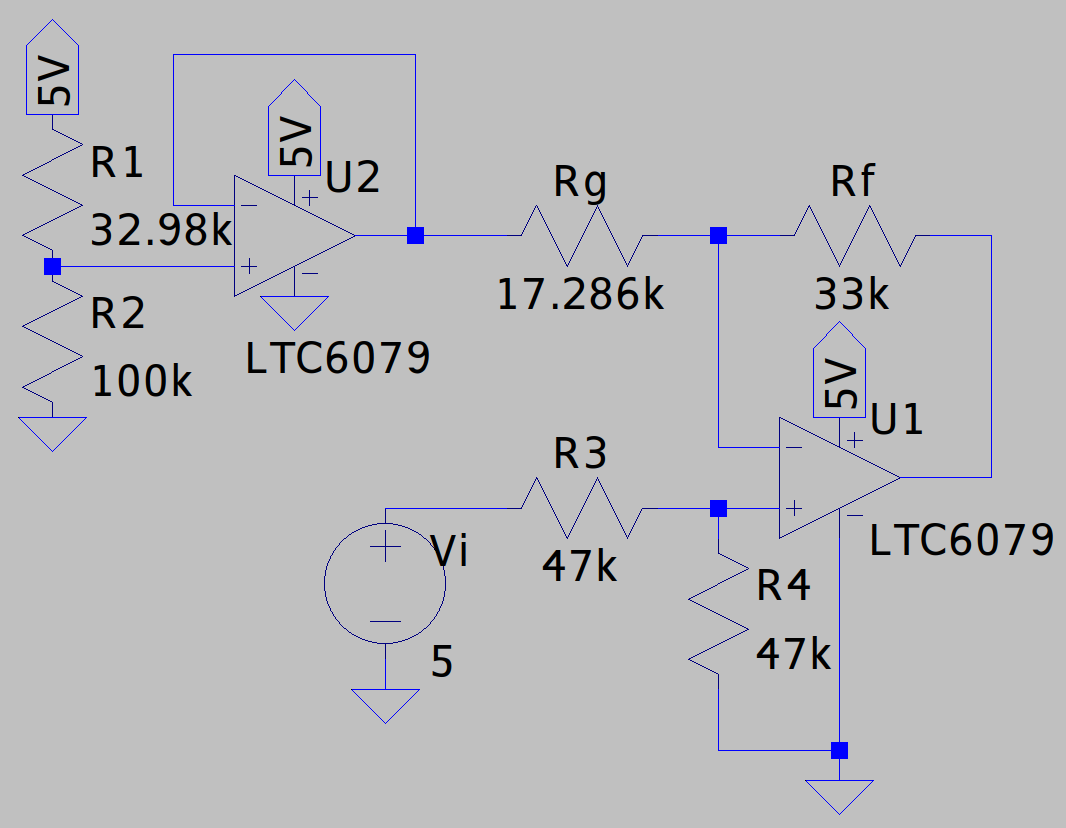
\includegraphics[width=0.4\textwidth]{batteryReader_circuitDiagram}
  \caption{Battery Reader Circuit Diagram}
  \label{fig:batteryReader_circuitDiagram}
\end{figure}

\subsection{Input and Output Range}

The input range is a voltage between 5.0 and 7.2 V, and the output is a voltage between 0.1 and 3.3 V. The common-mode input voltage of the op-amp should be taken into account,
meaning a voltage divider should be used at the positive input. Without a voltage divider, the battery voltage would be connected directly to the positive terminal of the op-amp,
and would be around $\SI{7.2}{V}$, which would violate the common-mode specification for the MCP \cite{datasheetMCP6242}. A voltage divider will therefore first half the voltage,
changing the input voltage to be between 2.5 to 3.6 V.

\pagebreak

\subsection{Design}

Resistor values may now be calculated:
\begin{itemize}
    \item The gain of the circuit $m = \frac{\SI{3.3}{V} - \SI{0.1}{V}}{\SI{3.6}{V} - \SI{2.5}{V}} = \SI{2.91}{V/V} = 1 + \frac{R_f}{R_g}$.
          To limit current in the feedback loop, ensure $\frac{\SI{3.3}{V}}{R_f + R_g} < \SI{100}{\micro\ampere} \therefore R_f + R_g > \SI{33}{\kilo\ohm}$.
          Choose $R_f = \SI{33}{\kilo\ohm} \therefore R_g = \SI{17.286}{\kilo\ohm}$. In order to adjust the gain, use a potentiometer and let $R_g = \SI{15}{\kilo\ohm} + \SI{4.7}{\kilo\ohm}$pot.
    \item To minimize current through the positive input voltage divider, ensure $\frac{\SI{7.2}{V}}{R_3 + R_4} < \SI{100}{\micro\ampere} \therefore R_3 + R_4 > \SI{72}{\kilo\ohm}$.
          Choose $R_3 = R_4 = \SI{47}{\kilo\ohm}$.
    \item If the voltage from the divider containing $R_1$ and $R_2$ is $V_{ref}$, then when $V_p = V_n = V_{in} = \SI{2.5}{V}$ and $V_{out} = \SI{0.1}{V}$,
          $\frac{V_n - V_{ref}}{R_g} + \frac{V_n - V_{out}}{R_f} = 0$ (found using a KCL) $\therefore V_{ref} = \SI{3.76}{V}$.
    \item Lastly, to calculate resistors $R_1$ and $R_2$, $V_{ref} = \SI{3.76}{V} = \SI{5}{V} \times \frac{R_2}{R_1 + R_2}$. Again, to limit current, choose $R_2 = \SI{100}{\kilo\ohm}$
          $\therefore R_1 = \SI{32.98}{\kilo\ohm}$. To adjust this offset voltage, choose $R_1 = \SI{27}{\kilo\ohm} + \SI{10  }{\kilo\ohm}$pot.
\end{itemize}